\section{Vista Física}
Se va a utilizar una arquitectura cliente servidor tipica, en la cual el backend y el acceso a la base de datos van a estar alojados en el mismo servidor y el frontend va a estar alojado en otro.
\begin{figure}[htbp]
          \centering
          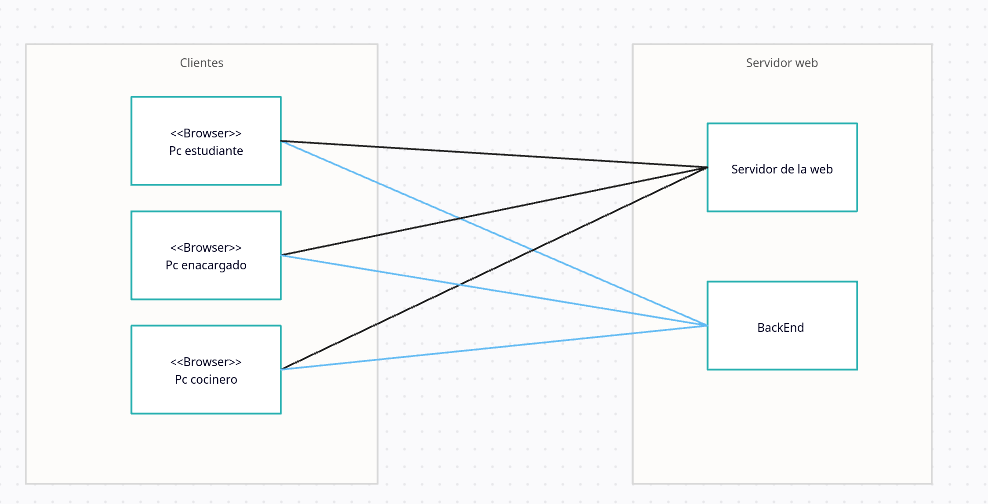
\includegraphics[width=0.9\textwidth]{img/Vista_fisica.png}
          \caption{Diagrama de la vista fisica}
          \label{fig:pysh}
        \end{figure}

En negro se marcaron las conexiones que se dan por primera vez para solicitar la pagina web al servidor. Luego la aplicación se comunicara todo el tiempo con el servidor backend mediante la API de la capa de servicio.

\newpage